First of all, let us examine the different ways by which
antibodies are naturally used by the immune system to combat
a pathogen infection. There are four of them, complementary of each other.

The key point here is that the antibodies allow for a specific recognition
of an antigen, and allow the immune system to act on it after it has
been detected. The antibodies on their own do not kill nor suppress any pathogen,
but act as the "recognition" part of the whole immune system.

\subsubsection{Antigen neutralization}

\begin{figure}[H]
    \begin{minipage}{0.55\textwidth}
        The most simple way antibodies can act against a pathogen is by
        \emph{neutralization} : the antibodies specific to an epitope of the
        antigen bind to this epitope and form together a complex that surround
        the pathogen \cite{langermans_antimicrobial_1994}.
        It is thus geometrically prevented to act as it normally would 
        by infecting the nearby cells.

        Antibodies acting in this manner are called \emph{neutralizing antibodies}
        or NAbs. The neutralized pathogen cannot approach the cell and
        bind to its surface receptors, thus making it ineffective. 
        The resulting complex can then be eliminated.
    \end{minipage}\hfill
    \begin{minipage}{0.35\textwidth}
        \centering
        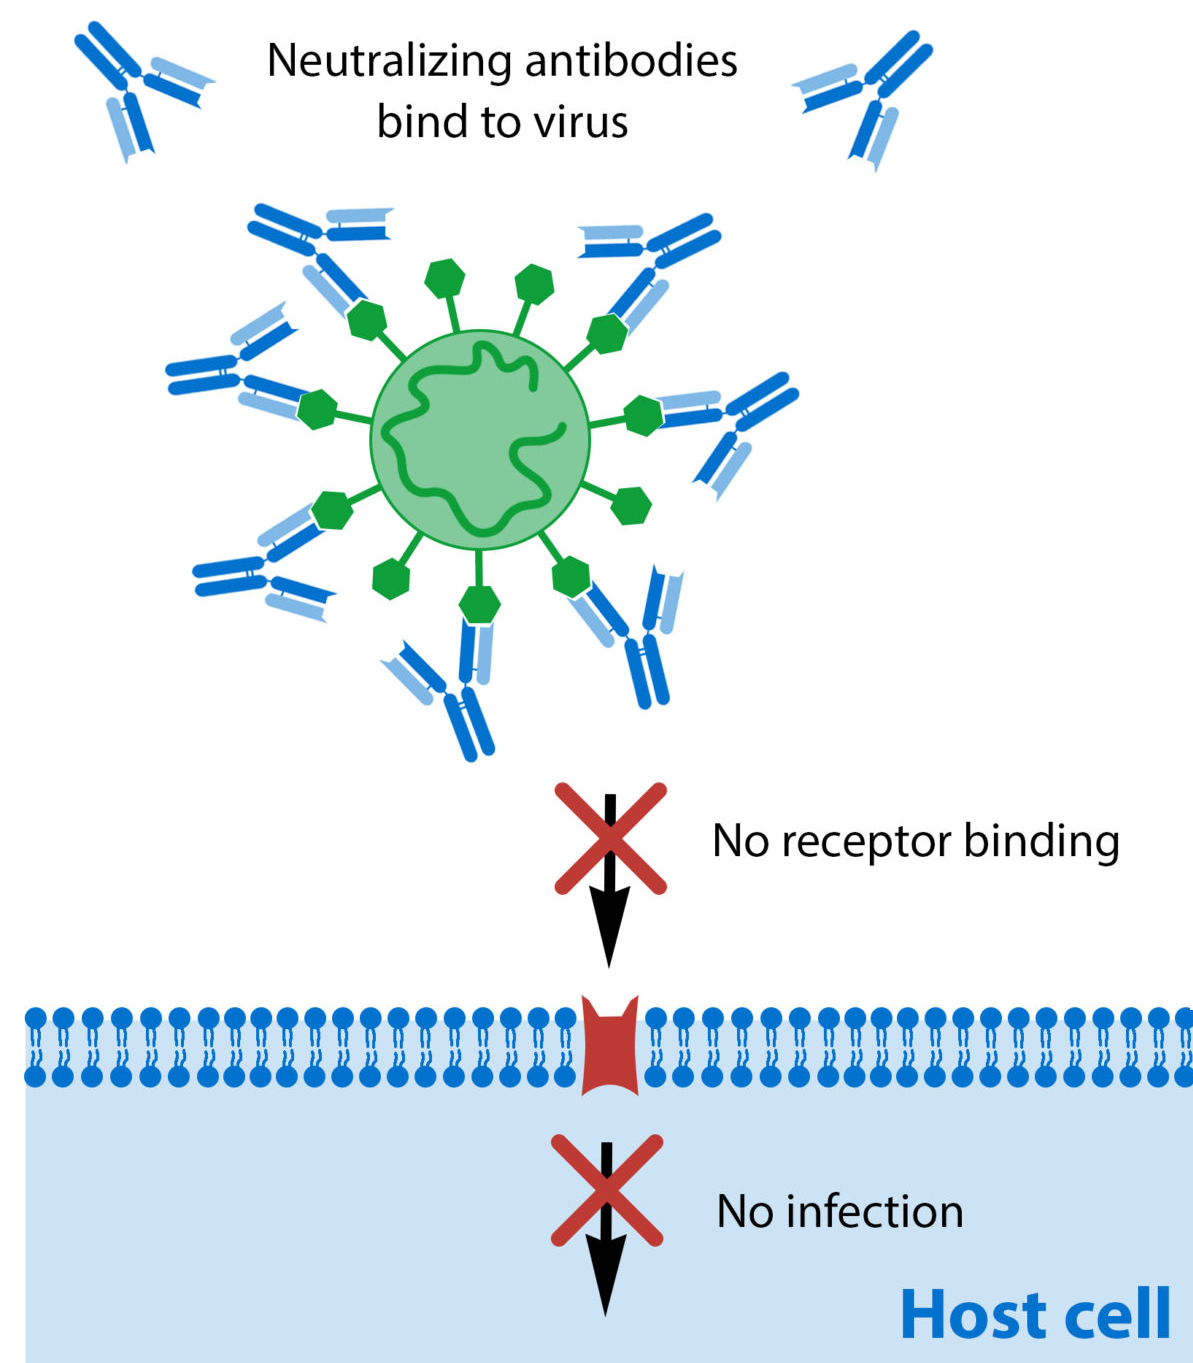
\includegraphics[width=\textwidth]{../Images/neutralization.png}   
        \caption{Neutralization of a pathogen by antibodies}
        \label{fig:neutralization}
    \end{minipage}
\end{figure}


\subsubsection{Antibody-Dependent Cellular Phagocytosis (ADCP)}

Another way by which antibodies help acting against a pathogen is very
close to neutralization. Indeed, once an antigen-antibody complex has been
created, some Fc receptor expressive immune effector cells can come into action
and act on the pathogen. 

\begin{figure}[H]
    \begin{minipage}{0.49\textwidth}
        \centering
        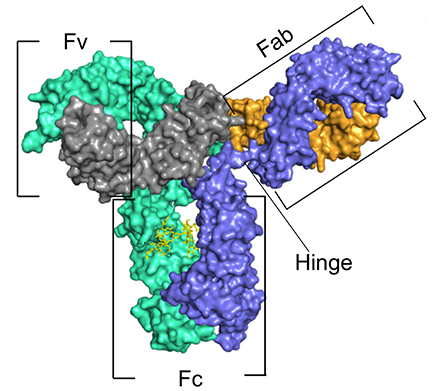
\includegraphics[width=0.9\textwidth]{../Images/antibody_domains.png}   
        \caption{The different domains of an immunoglobulin}
        \label{fig:antibody_domains}
    \end{minipage}\hfill
    \begin{minipage}{0.49\textwidth}
        \centering
        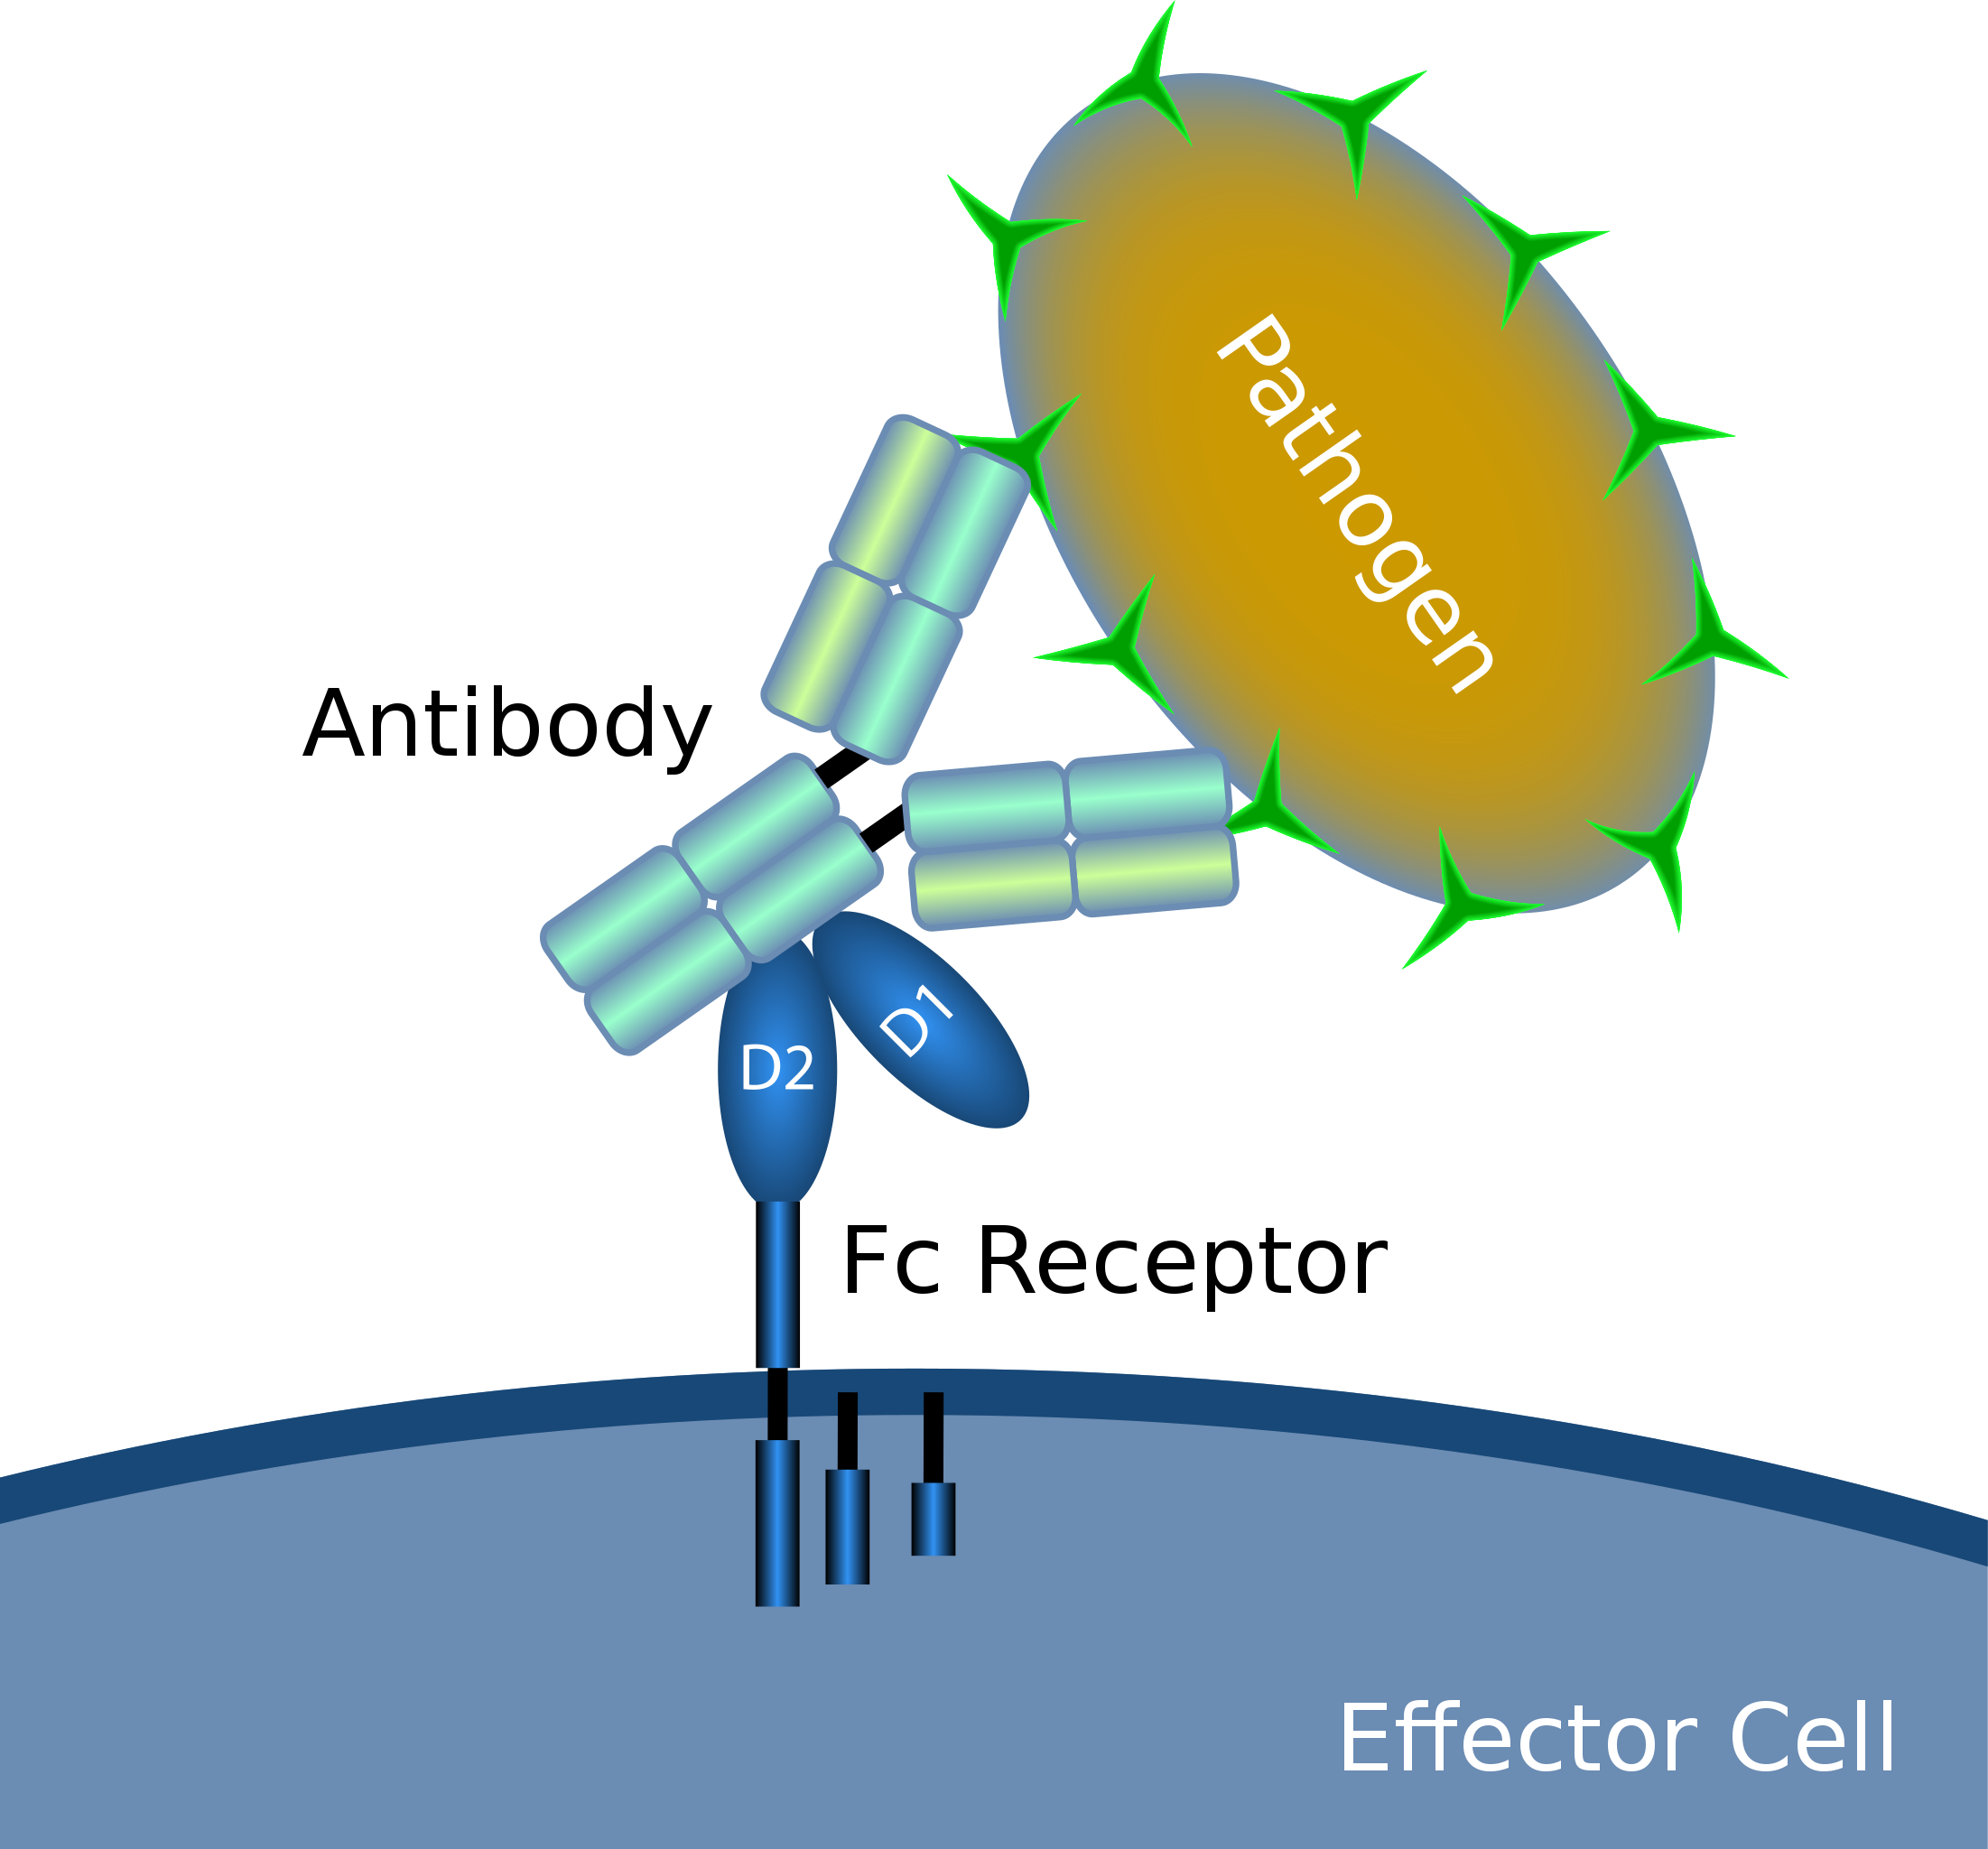
\includegraphics[width=0.9\textwidth]{../Images/Fc_receptor_interaction.png}   
        \caption{Interaction between the Fc receptor of an effector cell 
        and the Fc domain of an antibody attached to a pathogen}
        \label{fig:Fc_receptor_interaction}
    \end{minipage}
\end{figure}

Some cells, such as \emph{macrophages}, \emph{natural killer cells} or B lymphocytes, 
can bind to the Fc domain (shown on figure \ref{fig:antibody_domains})
of immunoglobulins attached to pathogens or infected -- or tumor -- cells
using their Fc receptors -- which are trans membrane proteins \cite{fridman_fc_1991}, 
as shown on figure \ref{fig:Fc_receptor_interaction}. 
The phagocytic or cytotoxic activity of the cell is then activated \cite{tay_antibody-dependent_2019}.
This mechanism allow for the precise elimination of antigenic material, the antibodies
permitting specific detection of the pathogen or undesirable cell, and the effector cells
killing and eliminating the antigen.

\begin{figure}[H]
    \begin{minipage}{0.49\textwidth}
        \centering
        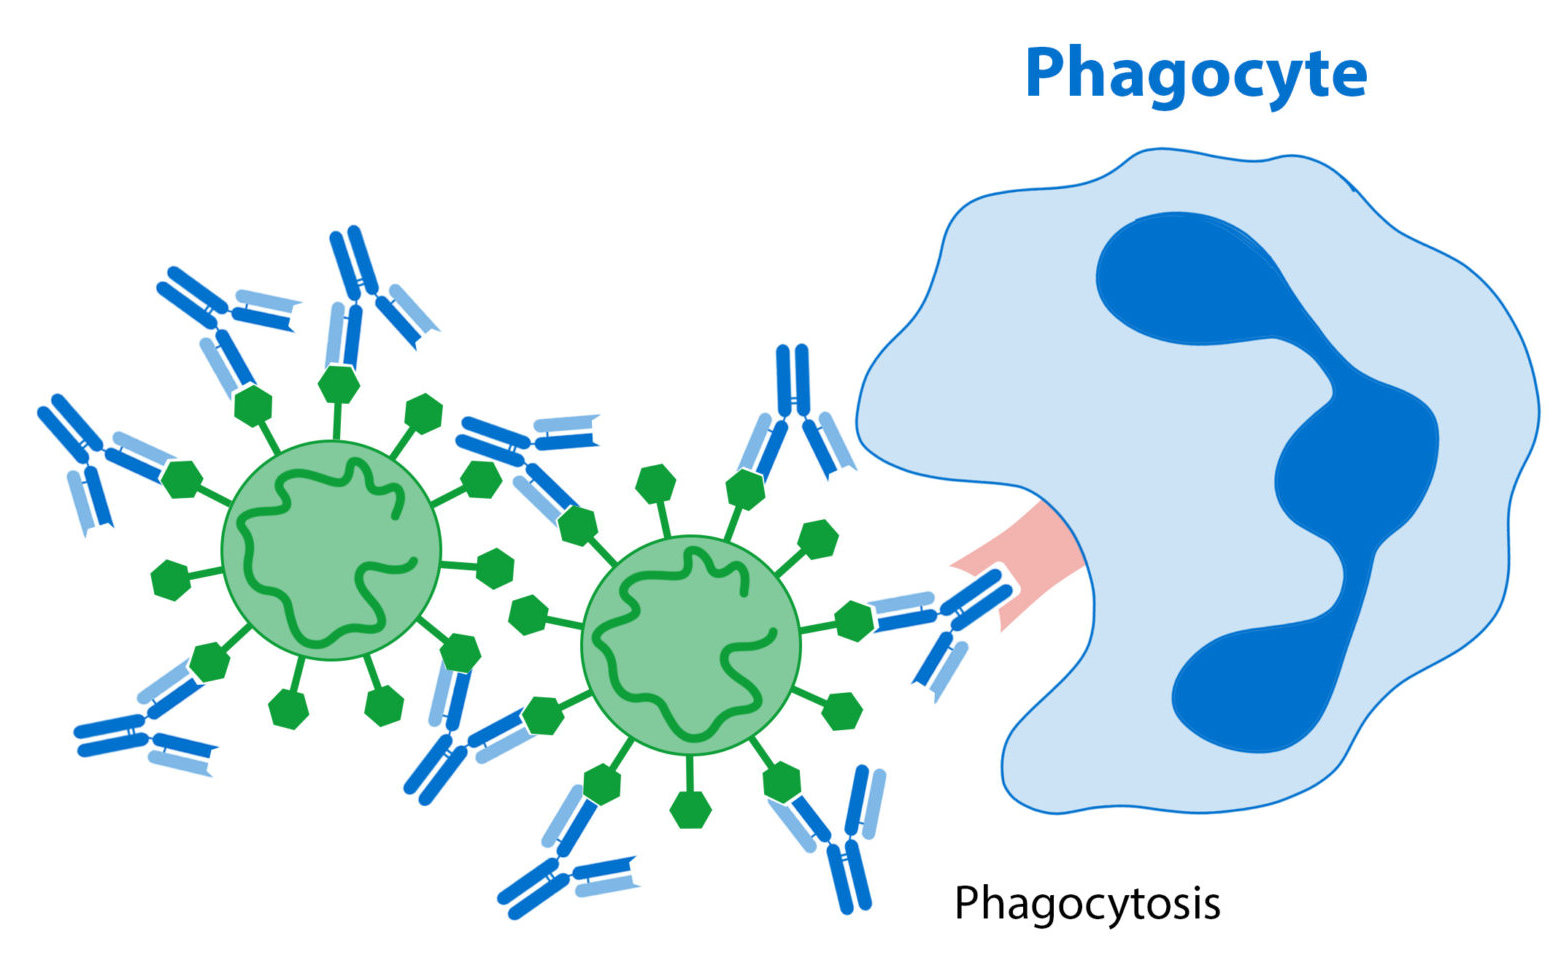
\includegraphics[width=0.9\textwidth]{../Images/phagocytosis.png}   
        \caption{Phagocytosis of a pathogen detected by antibodies}
        \label{fig:phagocytosis}
    \end{minipage}\hfill
    \begin{minipage}{0.49\textwidth}
        \centering
        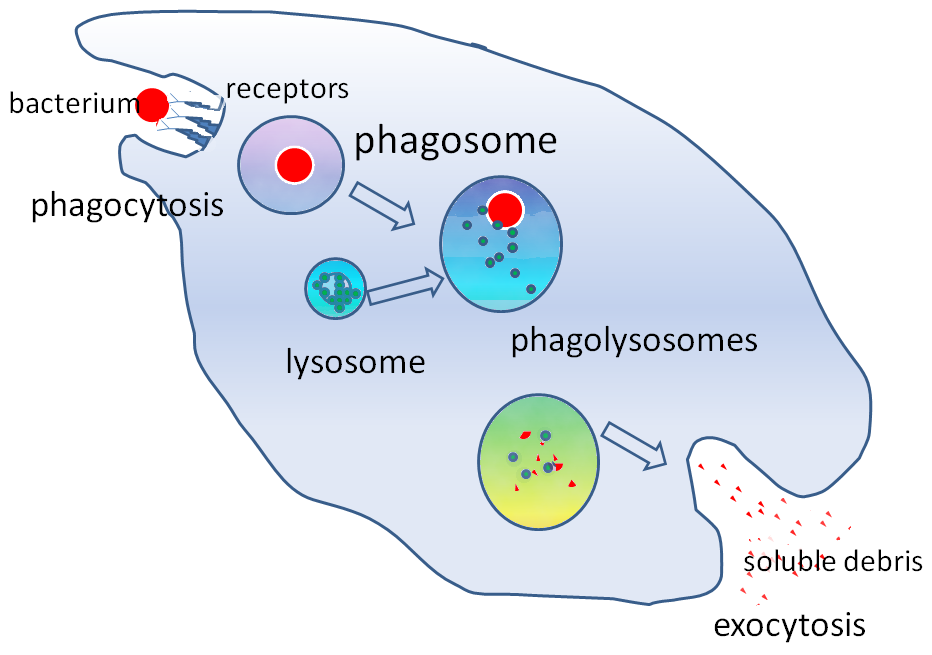
\includegraphics[width=0.9\textwidth]{../Images/phagocytosis_steps.png}   
        \caption{The steps of phagocytosis}
        \label{fig:phagocytosis_steps}
    \end{minipage}
\end{figure}

To speak more specifically about phagocytosis, this mechanism is of high importance
in a multicellular organism immune system ; it allows removal of large particles
(bigger than $0.5$ µm) such as dead cells, bacteria, mineral particles.

Phagocytosis occurs in multiple phases \cite{uribe-querol_phagocytosis_2020}
as seen on figure \ref{fig:phagocytosis_steps} : 
\begin{itemize}
    \item Detection of the particle that is going to be ingested
    \item Internalization and formation of a vacuole called \emph{phagosome}
    \item Maturation of the phagosome which is transformed in a \emph{phagolysosome}.
\end{itemize}

Degradation of the cell, bacteria or virus ingested is performed in the phagolysosome.
Indeed, the conditions inside the vacuole are extreme : the Ph is extremely acidic,
around $4,5$ due to the presence of many Vacuole ATPases \cite{uribe-querol_phagocytosis_2020},
the high concentration in $\text{H}^+$ ions being compensated for
by $\text{Cl}^-$ anions \cite{gordon_phagocytosis_2016}. 
Moreover, the phagolysosome membrane possesses the NADPH oxidase complex 
which produces Reactive Oxygen Species (ROS) like $\text{O}^{2-}$, which can then
dismutate to $\text{H}_2\text{O}_2$, which can itself react with $\text{Cl}^-$ ions
to form hypochlorous acid which is a highly active microbicidal substance while
being non-toxic to biological tissues \cite{eryilmaz_antimicrobial_2013}.
These conditions allow for the destruction of the cytoskeleton and the 
recycling of the components of the ingested cell.


It should be noted that although all types of cells can perform phagocytosis,
only professional cells such as macrophages, monocytes or dendritic cells can
do so with high efficiency. Finally, phagocytosis does not only act as an
immune response to an infection by a pathogen, but is a normal part of the
life cycle of tissues, as dead tissues cell are recycled 
in this way \cite{arandjelovic_phagocytosis_2015}.

\subsubsection{Antibody-Dependent Cell Cytotoxicity (ADCC)}

\subsubsection{Complement-Dependent Cell Cytotoxicity (CDCC)}
